%!TEX root = main.tex
\vspace{-3pt}
\section{Error Analysis\label{sec:error}}
\par On collecting and analyzing a number of crowdsourced segmentations (described in Section~\ref{dataset}), we found that common worker segmentation errors can be classified into three types: (1) \textbf{Semantic Ambiguity:} workers have differing opinions on whether particular regions belong to an object (Figure~\ref{error_examples} left: annotations around `flower and vase' when `vase' is requested); (2) \textbf{Semantic Mistake:} workers annotate the wrong object entirely (Figure~\ref{error_examples} right: annotations around `turtle' and `monitor' when `computer' is requested.); and (3) \textbf{Boundary Imperfection:} workers make unintentional mistakes while drawing the boundaries, either due to low image resolution, small area of the object, or lack of drawing skills (Figure~\ref{tile_demo} left: imprecision around the `dog' object).
\par Quality evaluation methods in prior work have largely focused on minimizing boundary imperfection issues. So, we first describe our novel aggregation-based algorithms designed to reduce boundary imperfections in Section~\ref{precision}. Next, in Section~\ref{perspective}, we discuss a preprocessing method eliminates semantic ambiguities and errors, also observed in prior work~\cite{Sorokin2008,Lin2014,Gurari2018}. We present our experimental evaluation in Section~\ref{sec:experiment}.% and compare them with existing retrieval-based methods in 
%\par %Out of the 46 objects in our dataset, 9 objects suffer from semantic ambiguity, 18 objects from semantic mistakes, and almost all objects suffer from some form of boundary imprecision to varying degrees. 
% \begin{figure*}[ht!]
%     \centering
%     \RawFloats
%     \begin{minipage}[t]{0.65\textwidth}
%     	\vspace{-20pt}
%         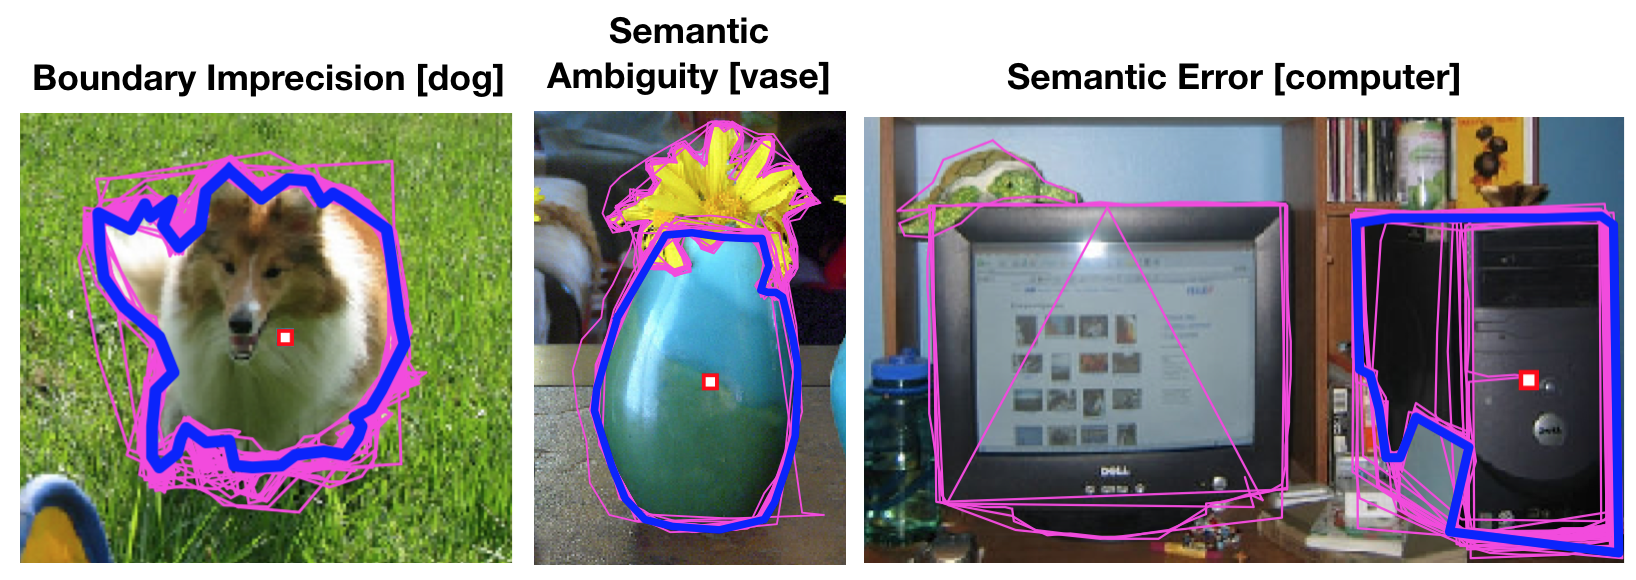
\includegraphics[width=\textwidth]{plots/error_examples.png} % second figure itself
%         \caption{Pink is the segmentation from individual workers. Blue solid line delineates the ground truth. The red boxed pointer indicates the task of interest shown to users.}
%         \vspace{-15pt}
%         \label{error_examples}
%     \end{minipage}
%     \begin{minipage}[t]{0.35\textwidth}
%     	\vspace{-25pt}
%         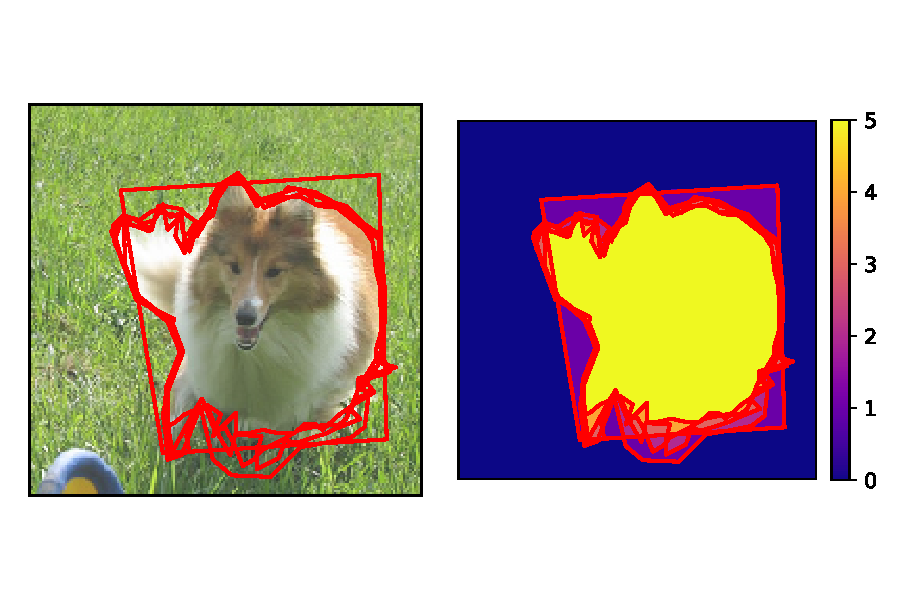
\includegraphics[width=\textwidth]{plots/tile_demo.pdf}
%         \vspace{-35pt}
%         \caption{Segmentation boundaries drawn by five workers in red. Right: Overlaid segmentation creates a masks where the color indicates the number of workers whose segmentation includes the tile region.}
%         \vspace{-20pt}
%         \label{tile_demo}
%     \end{minipage}\hfill
% \end{figure*}
\begin{figure}[h!]
    \centering
    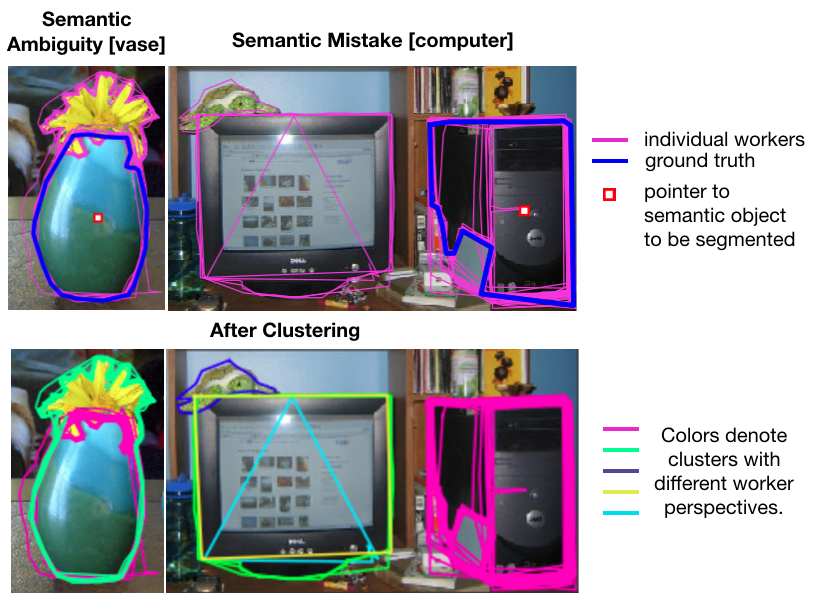
\includegraphics[width=0.85\textwidth]{plots/semantic_error_clust.png}
    \caption{\changes{Top: Examples of semantic ambiguities and mistakes. % where workers display different perspectives on what regions should be included as part of the object. %The pink segmentations are drawn by individual workers. The blue solid line delineates the ground truth. The red boxed pointer is the interface icon indicating the semantic object to be segmented. 
    Bottom: Examples of worker segmentations from different clusters.%, where different colors depict clusters representing different worker perspectives.
    }}
    \label{error_examples}
    \setlength{\abovecaptionskip}{-20pt}
\end{figure}